\documentclass[dvipdfmx,report,11pt]{jsbook}
\usepackage{package}
\setcounter{secnumdepth}{4}

\title{第1回(横山)}
\author{横山遥乙}
\date{\today}
\begin{document}
\newcommand{\ctext}[1]{\raise0.2ex\hbox{\textcircled{\scriptsize{#1}}}}
\newcommand{\sign}{\operatorname{sign}}
% \maketitle

%\tableofcontents

%%%%%%%%%%%%%%%%%%%%%%%%%%%%%%%%%%%%%%%%%%%%%%%%%%%%%%%%%%%%%%%%%%%%%%

\chapter{ニューラルネットワークとは}
\section{はじめに}
機械学習とは明治的にプログラムしなくても学習する能力をコンピュータに与える分野とされるが, そのうちニューラルネットワークは, 生物の学習メカニズムを図\ref{fig1}のように模倣した機械学習アルゴリズムである. より具体的に言えば, ある入力に対して重みをつけて出力情報を送り, それによる予測値$\hat{y}$と訓練データ$y$を比較することで, 再度重みを調整するという流れでそのネットワークを構成する.
\begin{figure}[H]
  \centering
    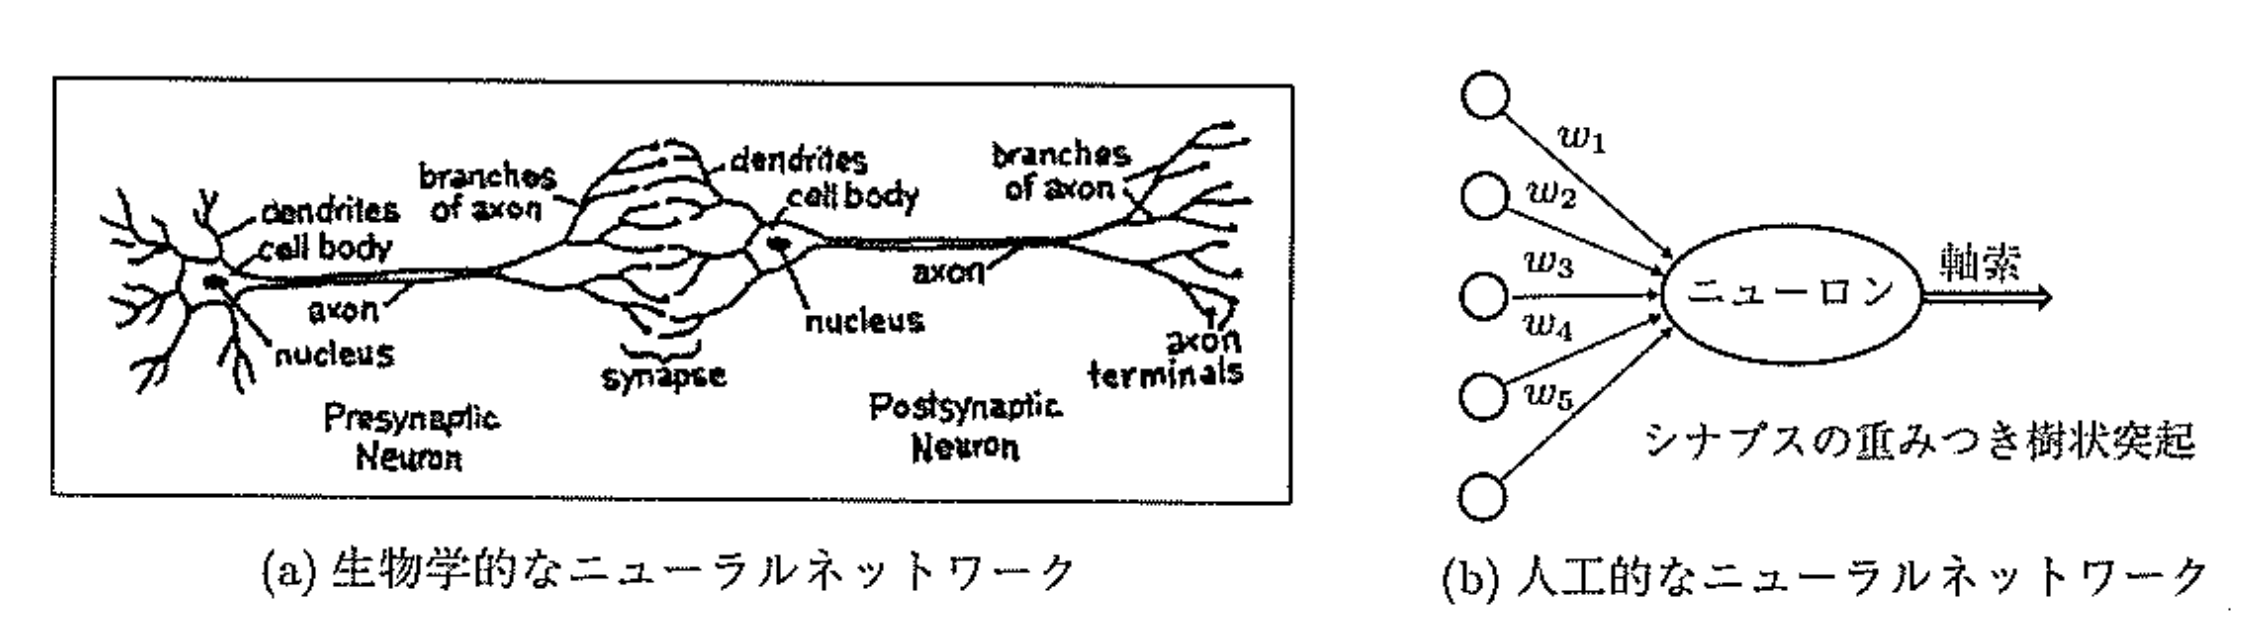
\includegraphics[width=0.8\linewidth]{figure/fig1.png}
    \caption{ニューロン間のシナプス結合}
    \label{fig1}
\end{figure}

従来の機械学習アルゴリズム(最小二乗回帰, ロジスティック回帰, etc.)と比べた場合, ニューラルネットワークの利点は
\begin{enumerate}
  \item 計算グラフのアーキテクチャ設計の選び方によって, データの応用領域の意味論的な知見を表現できるような, 高レベルの抽象化が可能.
  \item どの程度の訓練データや計算能力が利用できるかに応じて, アーキテクチャにニューロンを追加・消去し, モデルの複雑さを簡単に調整可能.
\end{enumerate}
ということが上がる. なお, 小さなデータセットの場合については, 従来の機械学習アルゴリズムの方が優位になることもあるので注意が必要(図\ref{fig2}).
\begin{figure}[H]
  \centering
    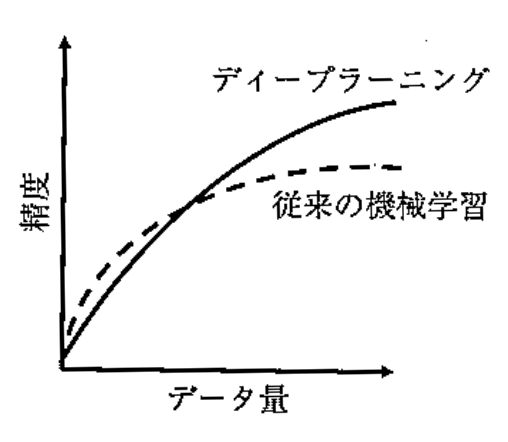
\includegraphics[width=0.3\linewidth]{figure/fig2.png}
    \caption{}
    \label{fig2}
\end{figure}

\section{ニューラルネットワークの基本的なアーキテクチャ}
最も単純なニューラルネットワークはパーセプトロンと呼ばれ, 図\ref{fig3}のように, ネットワークの層が一層で, 入力の集合を直接出力に写像するようなものを指す. また, ニューロンが層状に配置され, 入力層と出力層が複数の隠れ層によって隔てられているようなものは, 多層ニューラルネットワーク及び順伝播型ネットワーク(feed-forward network)と呼ばれている.


\subsection{単一の計算層: パーセプトロン}
いま, 個々の訓練データが$d$個の特徴量$\bm{X}=[x_1, \cdots, x_d]$と観測値2値のクラス変数$y\in\{-1,+1\}$の$(\bm{X},y)$で与えられる状況を考える. そして目標は訓練データ$(\bm{X},y)$を用いてニューラルネットワークを構成し, 未知の入力$x$に対して適切な予測値$\hat{y}$を出力することである. ニューラルネットワークを構成するにあたって, 重みを$\bm{W}=[w_1, \cdots, w_d]$のようにすれば, 各入力に対して$\bm{W}\cdot \bm{X}=\sum_{i=1}^d w_i x_i$として重みづけがなされる. そして出力においては2値分類を行うため, 符号関数$\operatorname{sign}$を用いれば, 予測値$\hat{y}$は以下のように計算される.
\begin{align}
  \hat{y}=\sign\{\bm{W}\cdot\bm{X}\}=\sign\{\sum_{j=1}^{d}w_jx_j\}
\end{align}
そして観測値$y$と予測値$\hat{y}$の間の誤差$E(\bm{X})=y-\hat{y}$を最小にするように, つまり誤差勾配が負となるように重み更新を行っていき, ニューラルネットワークを構成する.

\begin{figure}[H]
  \centering
    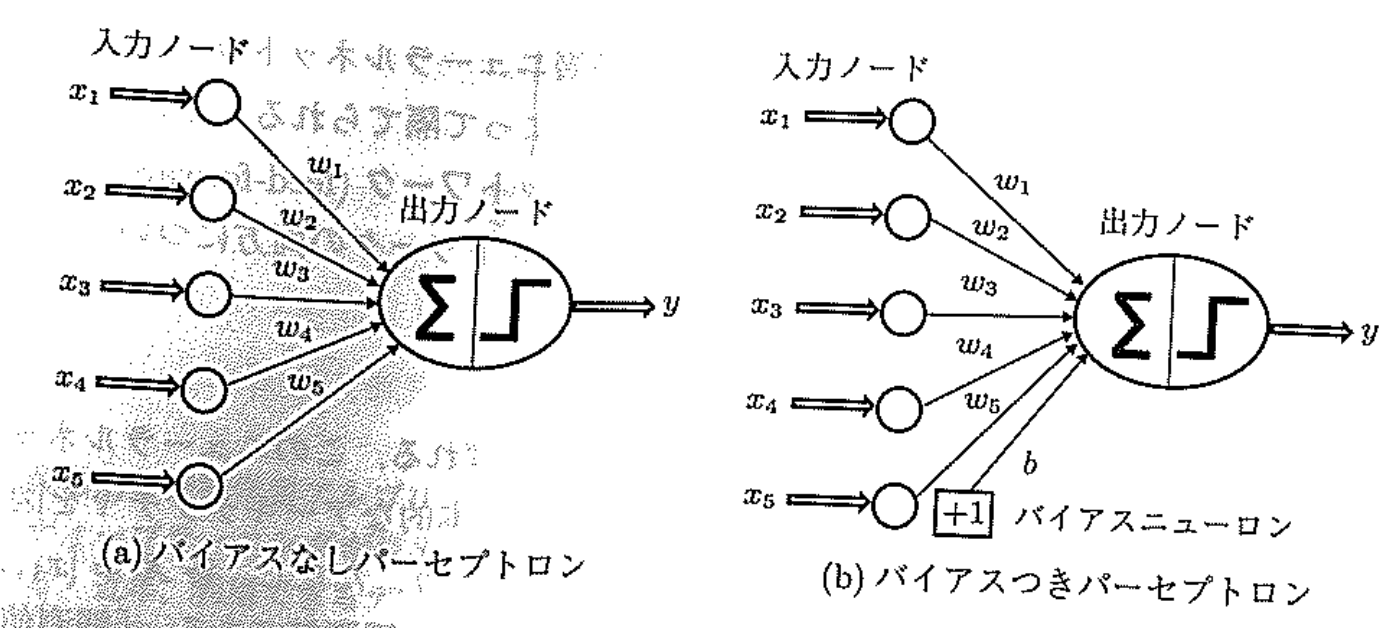
\includegraphics[width=0.5\linewidth]{figure/fig3.png}
    \caption{}
    \label{fig3}
\end{figure}

今回はクラスラベルに分類することが目標であったため, 入力に重みづけがされた値$\bm{W}\cdot \bm{X}$を符号関数で評価したが, これらは活性化関数と呼ばれ, 活性化関数の選び方によってニューラルネットワークの役割が決定されていく.

また, 多くの状況において予測にはバイアスと呼ばれる特徴量によらない不変な部分があり, 追加のバイアス$b$を組み込むことでこれを捉えることができる.
\begin{align}
  \hat{y}=\sign\{\bm{W}\cdot\bm{X}+b\}=\sign\{\sum_{j=1}^{d}w_jx_j+b\}
\end{align}



以上のことから, 特徴量とラベルのペアを含むデータセット$\mathcal{D}$内の全ての訓練データについて, パーセプトロンアルゴリズムの重み更新の目標を最小二乗形式
\begin{align}
  \text{Minimize}_{\bm{W}} L, \quad L=\sum_{(\bm{X},y)\in \mathcal{D}}(y-\hat{y})^2=\sum_{(\bm{X},y)\in \mathcal{D}}\left(y-\sign\{\bm{W}\cdot\bm{X}\}\right)^2\notag
\end{align}
で記述できる. これは損失関数(loss function)ともよばれ, ほとんどのニューラルネットワークの学習アルゴリズムは損失関数を使って定式化されている. しかしながら今回のように活性化関数が符号関数の場合, 微分不可能でありさらに定義いきの大部分で一定値を取るために, 微分可能な点での勾配は0となってしまう. そのため, パーセプトロンアルゴリズムでは暗黙的に, 各データごとの目的関数の勾配を滑らかに近似した
\begin{align}
  \nabla L_{\text{smooth}}=\sum_{(\bm{X},y)\in \mathcal{D}}(y-\hat{y})\bm{X}
\end{align}
を用いる.

では, 実際のニューラルネットワークの訓練アルゴリズムではどのように重みを更新しているかを考えると, それぞれの入力データ$\bm{X}$をネットワークに1つずつ(または小さなバッチで)与えて予測値$\hat{y}$を計算し, 誤差$E(\bm{X})=(y-\hat{y})$が最小となるようにニューラルネットワークの学習率を$\alpha$として
\begin{align}
  \bm{W}\Leftarrow \bm{W}+\alpha (y-\hat{y})\bm{X}\label{eq:1.4}\\
  \bm{W}\Leftarrow \bm{W}+\alpha E(\bm{X})\bm{X}
\end{align}
で更新がなされている(確率的勾配降下法). なお, ランダムに選択された訓練データの部分集合$S$からバッチを作って重みを更新するミニバッチ確率的勾配法は以下のように計算される.
\begin{align}
  \bm{W}\Leftarrow \bm{W}+\alpha \sum_{\bm{X}\in S}E(\bm{X})\bm{X}\label{eq:1.6}
\end{align}

% \subsubsection*{単純パーセプトロンの収束定理}
% 続いて重みの更新についてだが, パーセプトロンアルゴリズムは, 誤分類の数を最小限に抑えるように設計されていおり, その収束証明が与えられている.
% \begin{screen}
%   a
% \end{screen}
\begin{figure}[H]
  \centering
    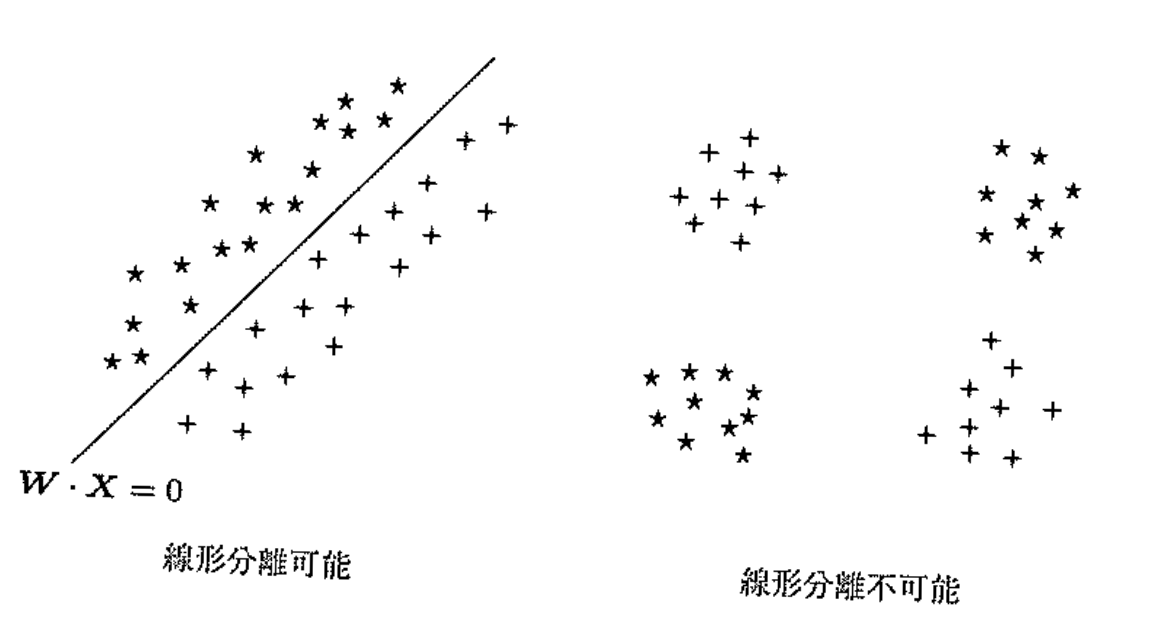
\includegraphics[width=0.5\linewidth]{figure/fig4.png}
    \caption{}
    \label{}
\end{figure}

\subsubsection{パーセプトロンはどのような目的関数を最適化しているか}
2値分類における誤分類数は, 訓練データ$(\bm{X}_i,y_i)$ごとに$0/1$損失関数の形で以下のように書ける.
\begin{align}
  L_{i}^{(0,1)}=\dfrac{1}{4}\left(y_i-\sign\{\bm{W}\cdot\bm{X}_i\}\right)^2=\dfrac{1}{2}\left(1-y_i\cdot \sign\{\bm{W}\cdot\bm{X}_i\}\right)\label{eq:1.7}
\end{align}
しかしこれは微分不可能であり, ニューラルネットワークは勾配に基づく最適化によって定義されるため, パーセプトロンの更新に対応する滑らかな目的関数を定義する必要がある. そこでパーセプトロンの更新には暗黙的にパーセプトロン基準(目的関数を滑らかなものに置き換えたもの)を最適化しているということが示されている. したがって, 式\eqref{eq:1.7}における符号関数を除去し, 正しい予測に対しては全ての損失が0となるようにすることで, 目的関数は以下のように定義することができる.
\begin{align}
  L_i=\operatorname{max}\{-y_i(\bm{W}\cdot \bm{X}_i),0\}
\end{align}
では, 実際に計算してみると
\begin{align*}
  \bm{W}\cdot\bm{X}_i=w_1x_1^i+\cdots+w_dx_d^i
\end{align*}
であり
\begin{align*}
  \dfrac{\partial L_i}{\partial w_1}&=-y_ix_1^i,\\
  &\vdots\\
  \dfrac{\partial L_i}{\partial w_d}&=-y_ix_d^i\\
  \Rightarrow \nabla_WL_i&=-y_i\bm{X}
\end{align*}
となるから, $\bm{W}-\alpha\nabla_WL_i=\bm{W}-y_i\bm{X}$となり, 式\eqref{eq:1.4}のパーセプトロン更新式と一致することが確かに確認できる.


\subsubsection{サポートベクトルマシンとの関係}
パーセプトロンは二章で扱う, サポートベクトルマシンで使われているヒンジ損失を平行移動したものとも捉えることができる. ヒンジ損失は
\begin{align}
  L_i^{SVM}=\operatorname{max}\{1-y_i(\bm{W}\cdot\bm{X}_i),0\}
\end{align}
で定義され, 最大値関数の中に定数を持って平行移動されている(図\ref{fig6}). この類似性をより理解するために式\eqref{eq:1.6}を
\begin{align}
  \bm{W}\Leftarrow \bm{W}+\alpha \sum_{(\bm{X},y)\in S^{+}}y\bm{X}
\end{align}
と書く($S^{+}$は$y(\bm{W\cdot\bm{X}})<0$を満たすような全ての誤分類された点$\bm{X}\in S$の集合). ここで, $S^+$における誤分類された点では, $\sign\{\bm{W}\cdot\bm{X}\}=0$となることはなく, 誤差値は$E(\bm{X})=(y-\sin\{\bm{W}\cdot\bm{X}\})\in\{-2,+2\}$となることがわかる. 従って, 誤分類された点については必ず$E(\bm{X})=2y$となり, 学習率に係数2を含めれば$y$に置き換えられる関係にあることがわかる. つまり, サポートベクトルマシン(SVM)では決定境界付近のほぼ正しい点も更新の対象にするのに対し, パーセプトロンで考えれば, 誤分類された点に対してのみ更新が行われるとみることができる.

\setcounter{figure}{5}
\begin{figure}[H]
  \centering
    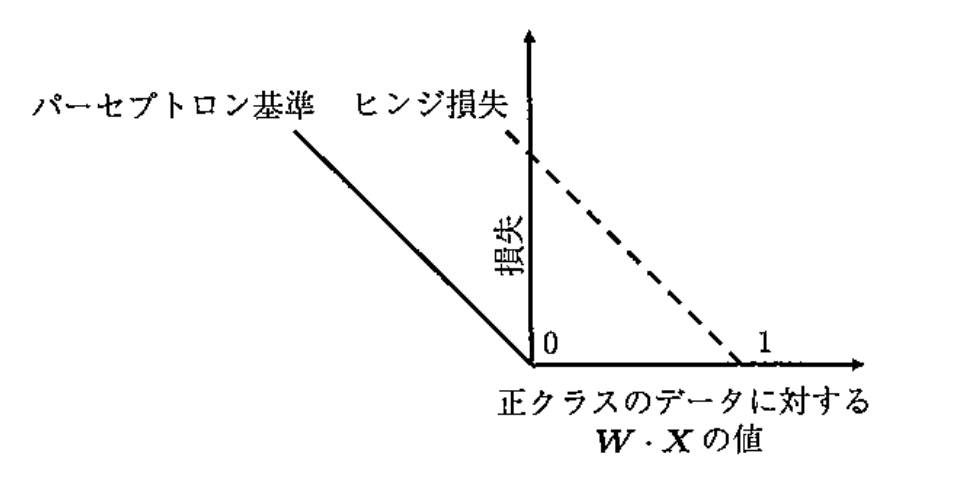
\includegraphics[width=0.5\linewidth]{figure/fig6.png}
    \caption{パーセプトロン基準とヒンジ損失}
    \label{fig6}
\end{figure}


\subsubsection{活性化関数と損失関数の選択}
パーセプトロンの場合, 2値のクラスラベルを予測したいという動機から, 活性化関数を符号関数に選んだが, 活性化関数を他のものにすることで, 様々な目的変数を予測できる. 以下に活性化関数の例を示す.
\begin{align*}
\begin{cases}
  \Phi(v)=\sign(v) & \text{(符号関数)}\quad\text{$\leftarrow$2値出力への写像}\\
  \Phi(v)=\dfrac{1}{1+e^{-v}} & \text{(シグモイド関数)}\quad\text{$\leftarrow$確率的解釈}\\
  \Phi(v)=\dfrac{e^{2v}-1}{e^{2v}+1} & \text{($\tanh$関数)}\quad \text{$\leftarrow$出力値が正と負の両方を取る確率的解釈}\\
  \Phi(v)=\operatorname{max}\{v,0\} & \text{(ReLu関数)}\quad \text{$\leftarrow$ 多層ニューラルネットワーク}\\
  \Phi(v)=\operatorname{max}\{\operatorname{min}[v,1],-1\} & \text{(ハード$\tanh$)}\quad \text{$\leftarrow$ 多層ニューラルネットワーク}\\
  \Phi(v)_i=\dfrac{\exp(v_i)}{\sum_{j=1}^k\exp(v_j)} & (ソフトマックス関数) \quad \text{$\leftarrow$出力を確率に変換する}
\end{cases}
\end{align*}
\setcounter{figure}{7}
\begin{figure}[H]
  \centering
    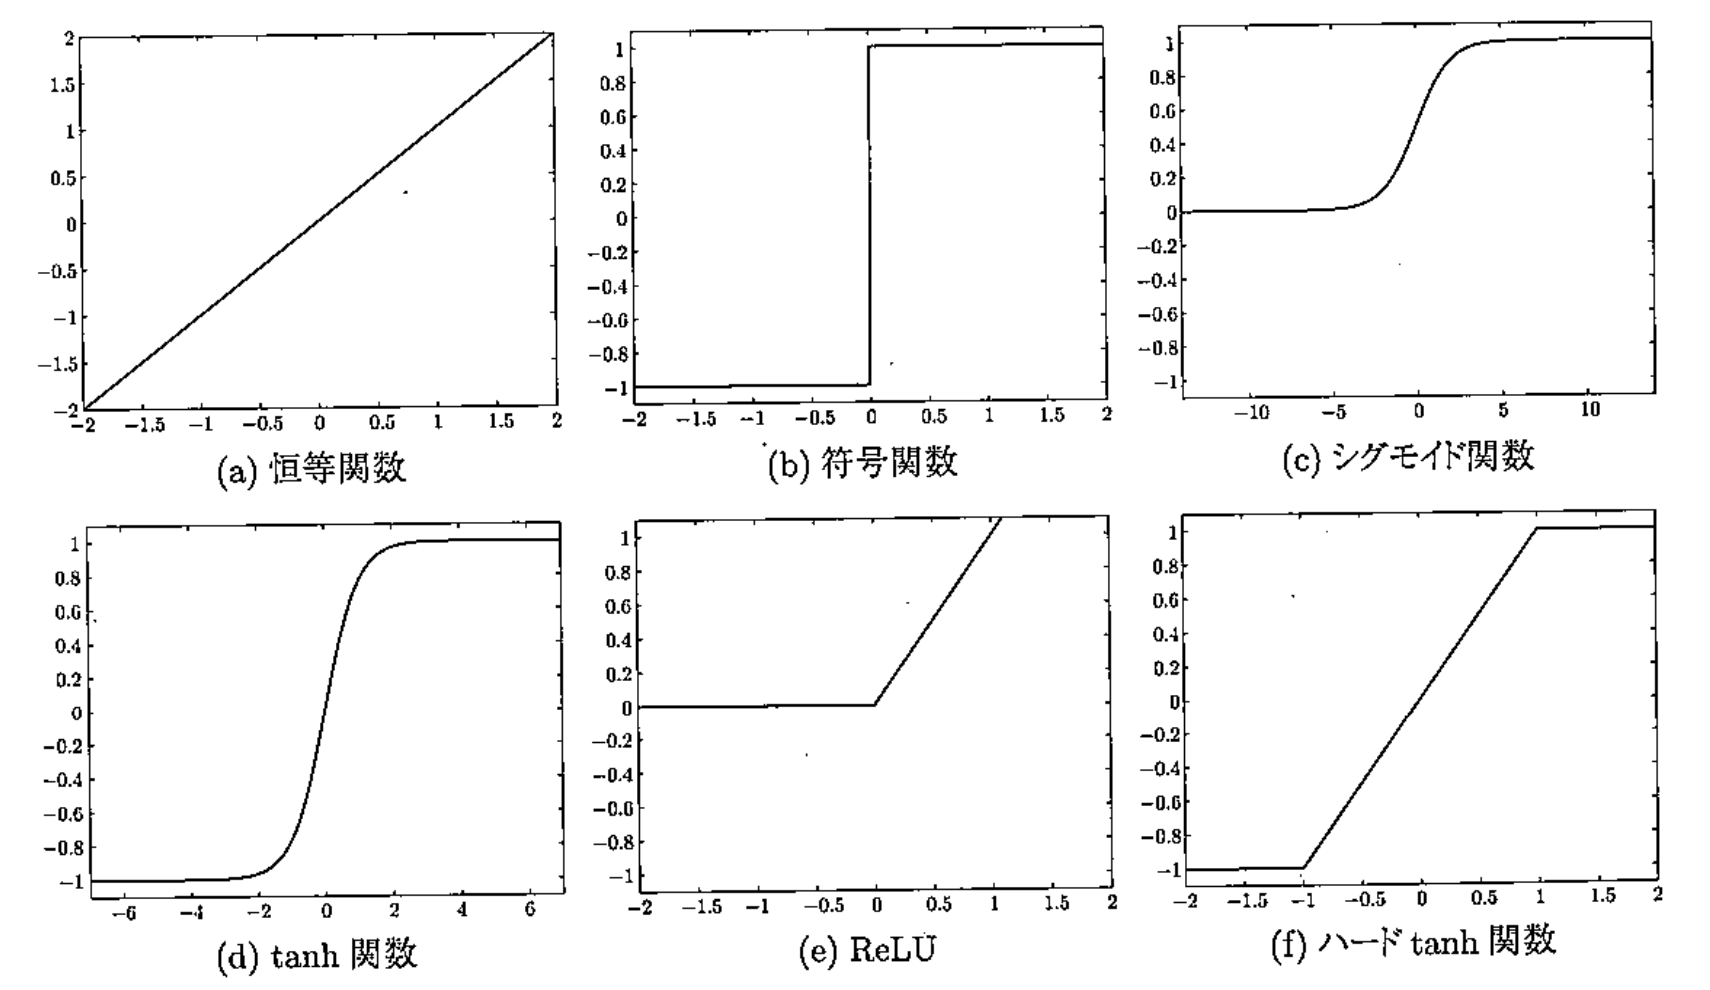
\includegraphics[width=0.8\linewidth]{figure/fig8.png}
    \caption{}
    \label{fig8}
\end{figure}
\setcounter{equation}{11}

\setcounter{subsubsection}{4}
\subsubsection{損失関数の選択}
\setcounter{equation}{13}
\begin{itemize}
  \item 目的変数が2値の場合(ロジスティック回帰)
  \begin{align}
    L=-\log(1+\exp(-y\cdot \hat{y}))
  \end{align}
  \item 目的変数がカテゴリの場合
  \begin{align}
    L=-\log(\hat{y}_r)
  \end{align}
\end{itemize}

\subsubsection{活性化関数の有用な導関数}
ニューラルネットワークでは, 活性化関数を用いた勾配降下法が重要な役割を演じるため, それぞれの導関数を示しておく.
\begin{enumerate}
  \item 恒等活性化関数と符号活性化関数\\
  恒等活性化関数は全ての場所で1であり, 符号活性化関数は$v=0$で不連続で微分不可能でそれ以外で0である. したがって, 導関数は常に0. (損失関数としてつかわれることはほとんどない.)
  \item シグモイド活性化関数\\
  $o$を$v$を引数とするシグモイド関数の出力とする.
  \begin{align}
    o=\dfrac{1}{1+\exp(-v)}
  \end{align}
  この導関数は
  \begin{align}
    \dfrac{\partial o}{\partial v}&=\dfrac{\exp(-v)}{(1+\exp(-v))^2}\\
    &=o(1-o)
  \end{align}
  となり, 出力を用いて記載できることがわかる.
  \item $\tanh$活性化関数\\
  \begin{align}
    o=\dfrac{\exp(2v)-1}{\exp(2v)+1}
  \end{align}
  この導関数は
  \begin{align}
    \dfrac{\partial o}{\partial v}&=\dfrac{4\exp(2v)}{(\exp(2v)+1)^2}\\
    &=1-o^2
  \end{align}
  となることがわかる.
  \item ReLU活性化関数とハード$\tanh$活性化関数\\
  ReLUの偏導関数は引数の値が非負であれば1, そうでなければ0. ハード$\tanh$の導関数は引数の値が$[-1,+1]$の場合は1をとり, それ例外では0を取る
\end{enumerate}
\begin{figure}[H]
  \centering
    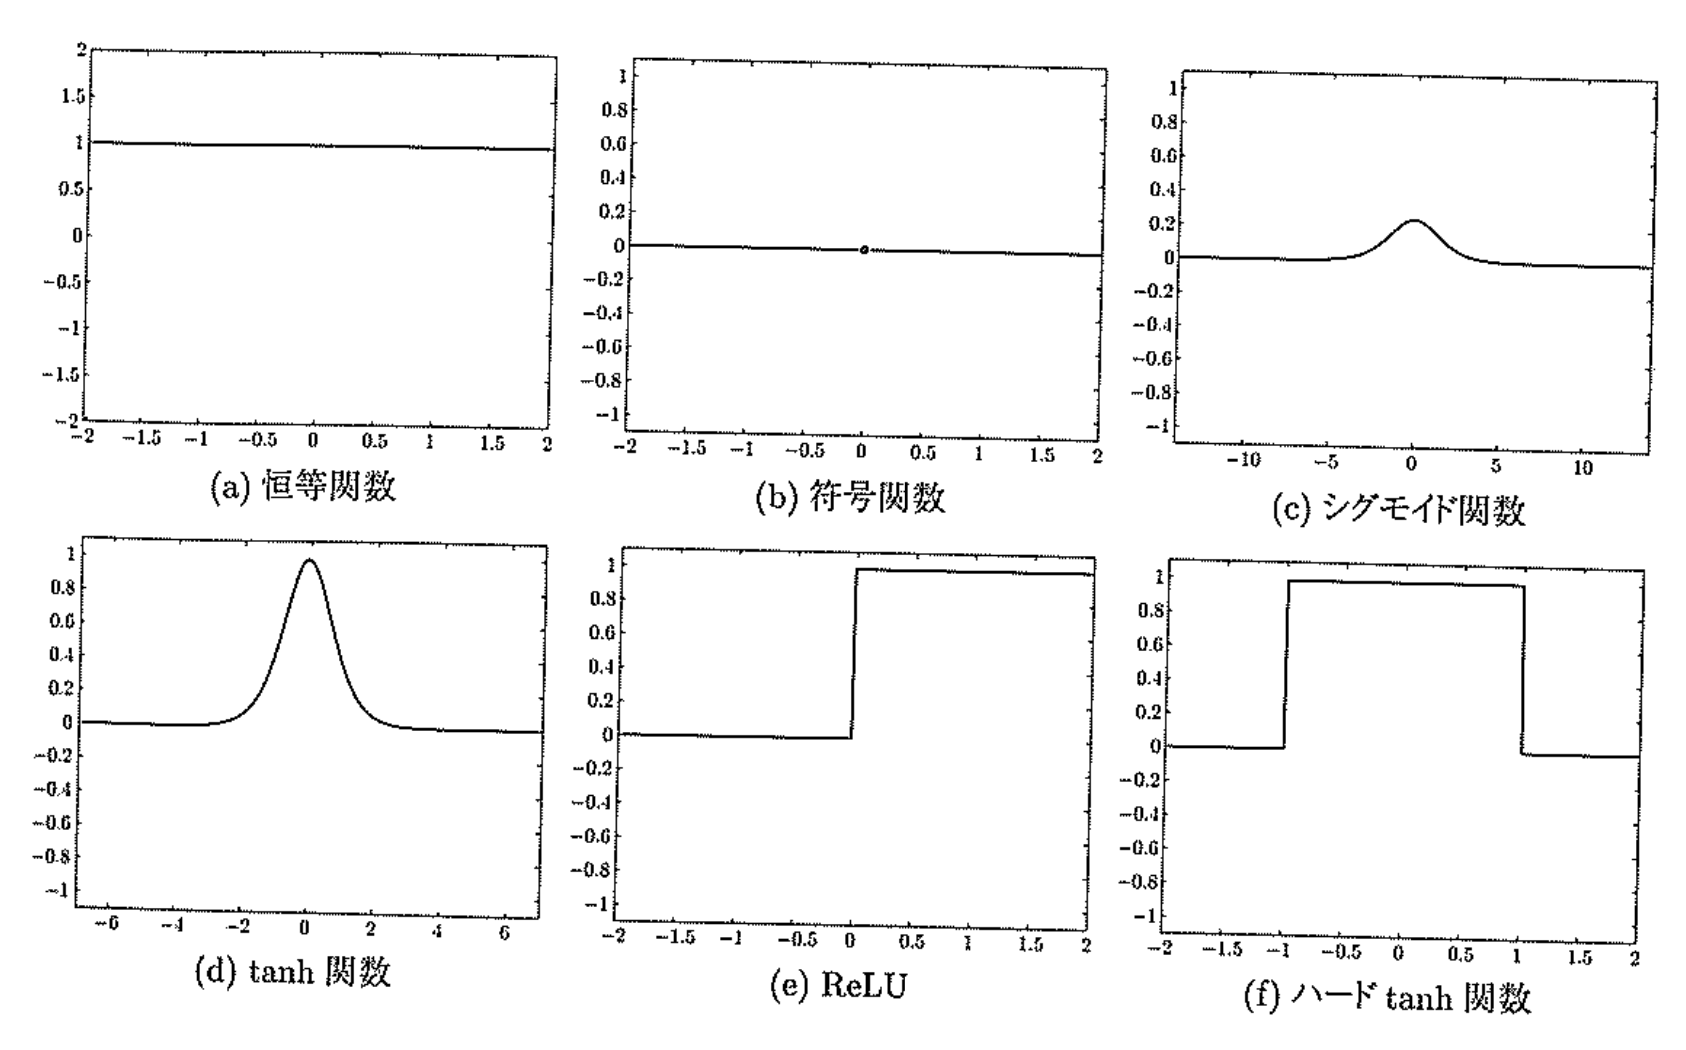
\includegraphics[width=0.7\linewidth]{figure/fig10.png}
    \caption{様々な活性化関数の導関数}
    \label{fig10}
\end{figure}

\subsection{多層ニューラルネットワーク}
多層ニューラルネットワークは, 図\ref{fig11}のように, 入力層と出力層の間に複数の中間層をもち, パーセプトロンでは出力層のみで行なっていた計算を中間層でも行う. いま, ニューラルネットワークの$k$個の層がそれぞれ$p_1, \cdots, p_k$個のユニットを含み, 入力が$x_1, \cdots, x_d$の場合, 入力層と1番目の隠れ層の間の重みは$p_r\times p_{r+1}$行列$W_1$で表され, $r$番目の隠れ層と$r+1$番目の隠れ層の間の重みは$p_r\times p_{r+1}$行列$W_r$で表される. そして最後の出力層が$o$個のノードを含む場合, 最後の行列$W_{k+1}$のサイズは$p_k\times o$となる. これを踏まえれば, $d$次元の入力ベクトルは以下のように再帰的に出力に変換される.
\begin{align*}
  \bm{h}_1&=\Phi(\bm{W}_1^T\bm{x})\\
  \bm{h}_{p+1}&=\Phi(\bm{W}_{p+1}^T\bm{h}_p)\\
  o&=\Phi(W_{k+1}^T\bm{h}_k)
\end{align*}

\begin{figure}[H]
  \centering
    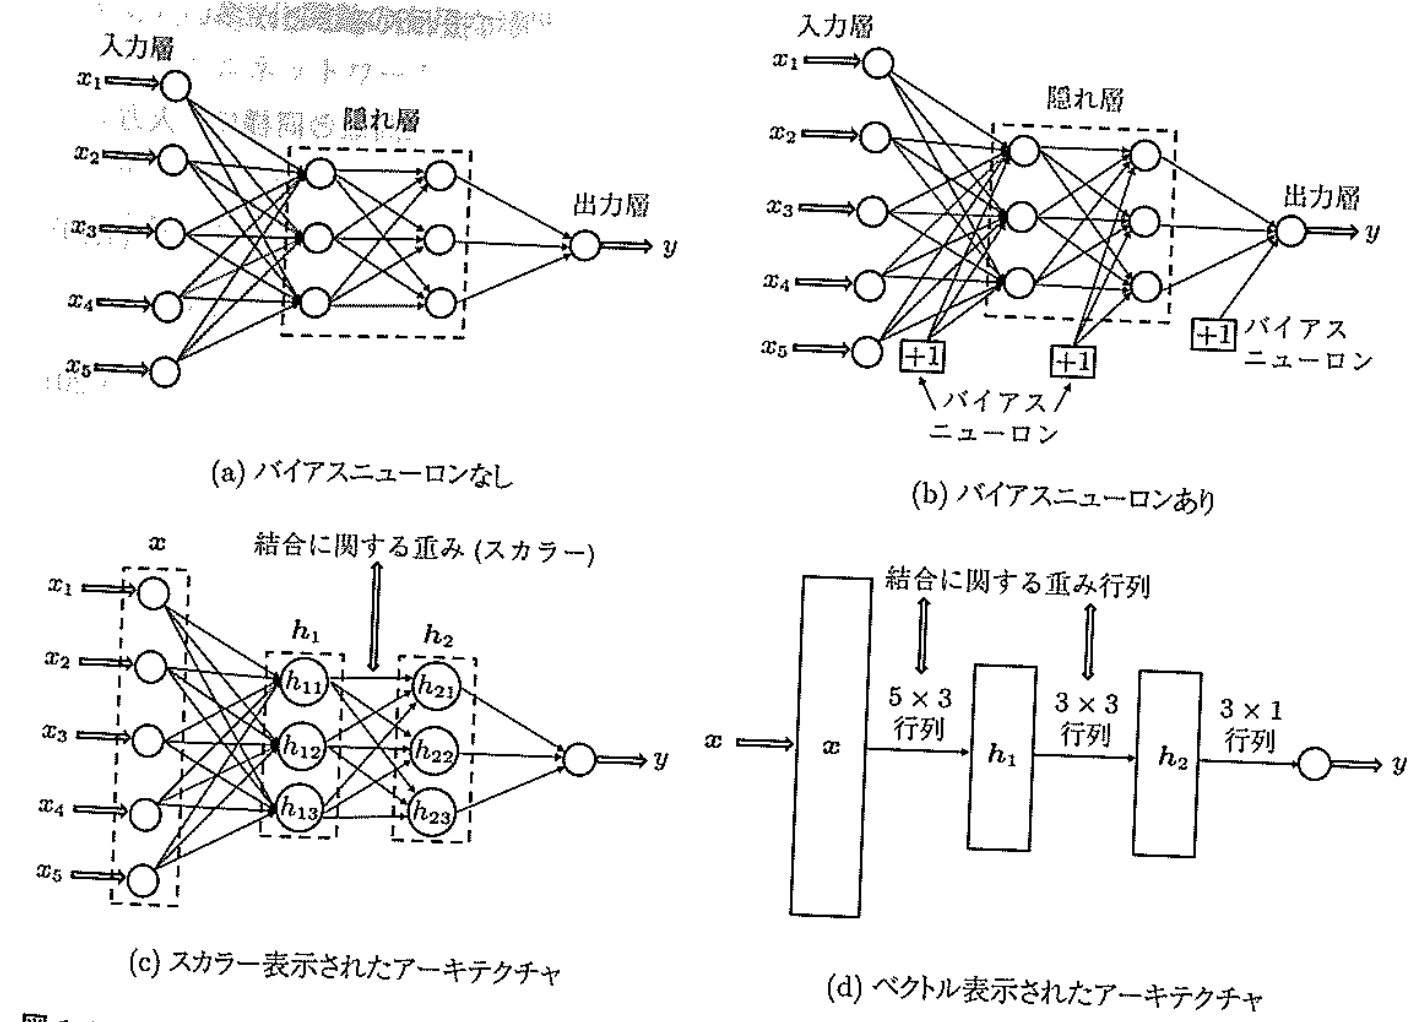
\includegraphics[width=0.6\linewidth]{figure/fig11.png}
    \caption{}
    \label{fig11}
\end{figure}
なお, ここでは順伝播型の古典的なアーキテクチャを示したが, 次元削減や畳み込みニューラルネットワークによって応用領域に沿った中間層アーキテクチャの設計がなされている.

\section{誤差逆伝播法によるニューラルネットワークの訓練}
\subsection{誤差逆伝播法}
重みの更新をするにあたって, 単一層ニューラルネットワークでは, 損失関数が直接重みの関数として計算できたことから, 学習の過程は比較的簡単であったが, 多層ネットワークの場合, 損失が前の層の重みの複雑な合成関数になるため, 更新が難しくなる. そこで用いられるのが誤差逆伝播法である.

誤差逆伝播法は
\begin{align}
  \dfrac{\partial L}{\partial w_{(h_{r-1},h_r)}}=\dfrac{\partial L}{\partial o}\cdot\left[\dfrac{\partial o}{\partial h_k}\Pi_{i=r}^{k-1}\dfrac{\partial h_{i+1}}{\partial h_i}\right]\dfrac{\partial h_r}{\partial w_{(h_{r-1},h_r)}}
\end{align}
で記述できる. これはネットワーク上に単一の経路しかないと仮定しているが, 複数の経路の勾配の計算には, 多変数連鎖率を用いて
\begin{align}
  \dfrac{\partial L}{\partial w_{(h_{r-1},h_r)}}=\underbrace{\dfrac{\partial L}{\partial o}\cdot\left[\sum_{[h_r, h_{r+1}, \cdots, h_k,o]\in \mathcal{P}}\dfrac{\partial o}{\partial h_k}\Pi_{i=r}^{k-1}\dfrac{\partial h_{i+1}}{\partial h_i}\right]}_{\Delta(h_r,o)=\frac{\partial L}{\partial h_r}}\dfrac{\partial h_r}{\partial w_{(h_{r-1},h_r)}}\label{eq:1.23}
\end{align}
として一般化できる($\mathcal{P}$は$h_r$から$o$までの経路の集合). 

では\eqref{eq:1.23}をどのようにして計算するかを考えると, ニューラルネットワークの計算グラフには巡回路がないことから, 全ての考えうる経路に対して
\setcounter{equation}{24}
\begin{align}
  \Delta\left(h_r, o\right)=\frac{\partial L}{\partial h_r}=\sum_{h: h_r \Rightarrow h} \frac{\partial L}{\partial h} \frac{\partial h}{\partial h_r}=\sum_{h: h_r \Rightarrow h} \frac{\partial h}{\partial h_r} \Delta(h, o)
\end{align}
と計算できる. このとき, 活性化関数を適用する直前に隠れユニット$h$で計算された値を$a_h$とすれば
\begin{align}
  \frac{\partial h}{\partial h_r}=\frac{\partial h}{\partial a_h} \cdot \frac{\partial a_h}{\partial h_r}=\frac{\partial \Phi\left(a_h\right)}{\partial a_h} \cdot w_{\left(h_r, h\right)}=\Phi^{\prime}\left(a_h\right) \cdot w_{\left(h_r, h\right)}
\end{align}
となり, 更新式は
\begin{align}
  \Delta(h_r, o)=\sum_{h:h_r\Rightarrow h}\Phi'(a_h)\cdot w_{(h_r,h)}\cdot\nabla(h,o)
\end{align}
となる. また, 式\eqref{eq:1.23}の末尾は
\begin{align}
  \dfrac{\partial h_r}{\partial w_{(h_{r-1}, h_r)}}=h_{r-1}\cdot\Phi'(a_{h_r})
\end{align}
と計算できる.

% \section{ニューラルネットワークの訓練の実践上の課題}


% \bibliographystyle{unsrt}
% \bibliography{Reference}
\end{document}